% !TEX root =  centrtutorial.tex
\begin{frame}
  \frametitle{Betweenness Centrality ? Incremental and Faster}
  \centering
  \vfill
  {\huge Meghana Nasre, Matteo Pontecorvi, Vijaya Ramachandran}
  \vfill
  {\large MFCS '14: Mathematical Foundations of Computer Science}
\end{frame}

\begin{frame}
  \frametitle{Path Dependency}
  
  \begin{itemize}
    \item Pair dependency of $(s,w)$ on $v$:
      \[\dep_{st}(w)=\frac{\paths_{sw}(v)}{\paths_{sw}}\]
    \item Dependency of a node $s$ on another node $v$:
      \[\dep_s(v)=\sum_{t \in V}\dep_{st}(w)\]
    \item Can be computed recursively:
    \[
    \dep_s(v)=\sum_{w \mid v \in \pred_s(w) } \frac{\paths_{sv}}{\paths_{sw}} \left( 1 + \dep_{s}(w) \right)
    \]
    \item Betweenness can be expressed as function of dependencies:
      \[ \betw(v) = \sum_{s \neq v} \dep_s(v) \]
  \end{itemize}
  
  \begin{figure}[H]
    \centering
    
\includegraphics[scale=1]{imgs/path-dependency}
  \end{figure}
  
\end{frame}

\begin{frame}
  \frametitle{Main Result}

  \begin{figure}[H]
    \centering
    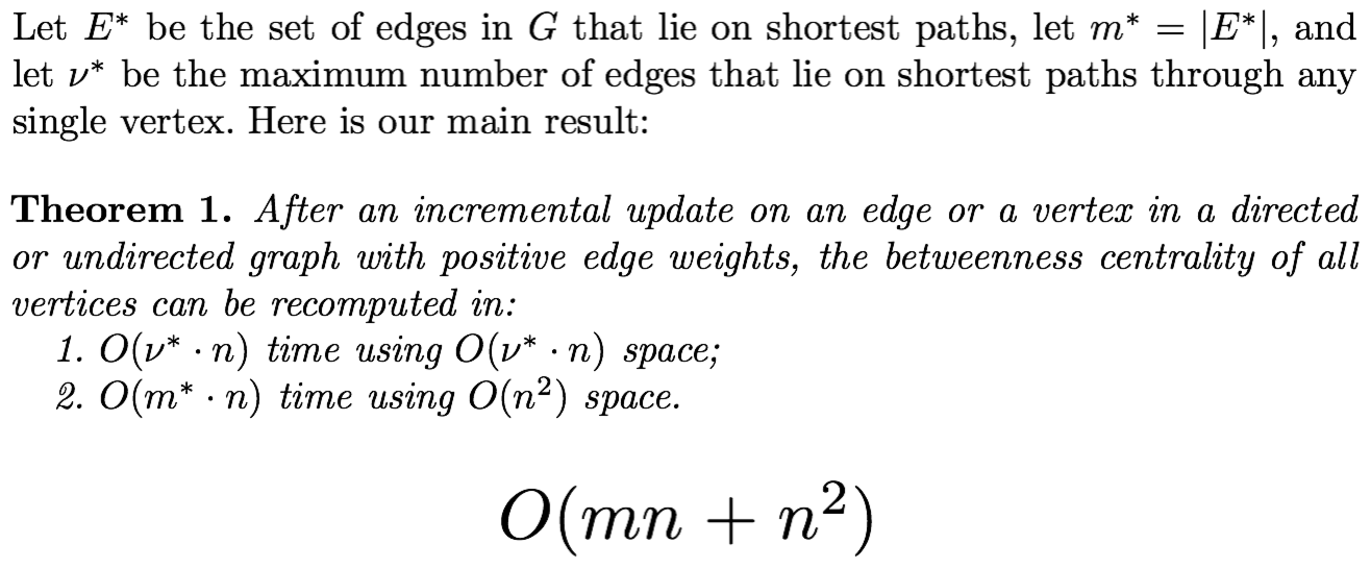
\includegraphics[width=\textwidth]{imgs/npr14-main-result}
  \end{figure}
  
\end{frame}

\begin{frame}
  \frametitle{Lemmas}

  \begin{figure}[H]
    \centering
    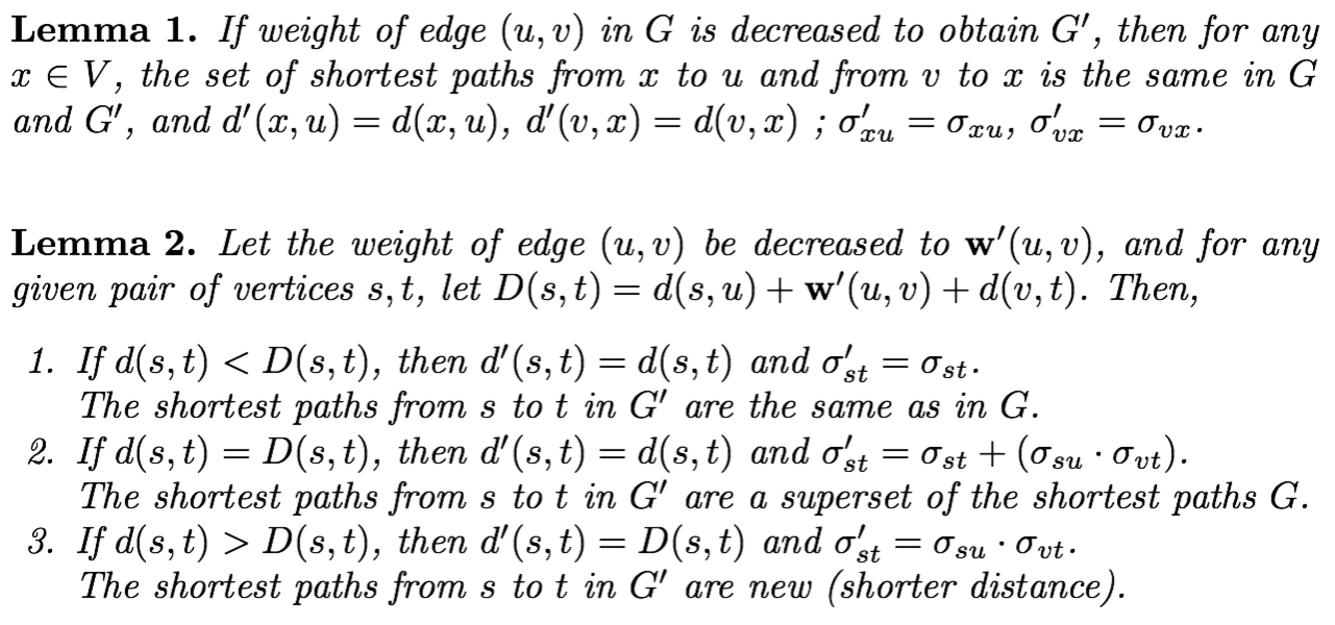
\includegraphics[width=\textwidth]{imgs/npr14-lemmas}
  \end{figure}
  
\end{frame}

\begin{frame}
  \frametitle{SSSP DAG Update}

  \begin{figure}[H]
    \centering
    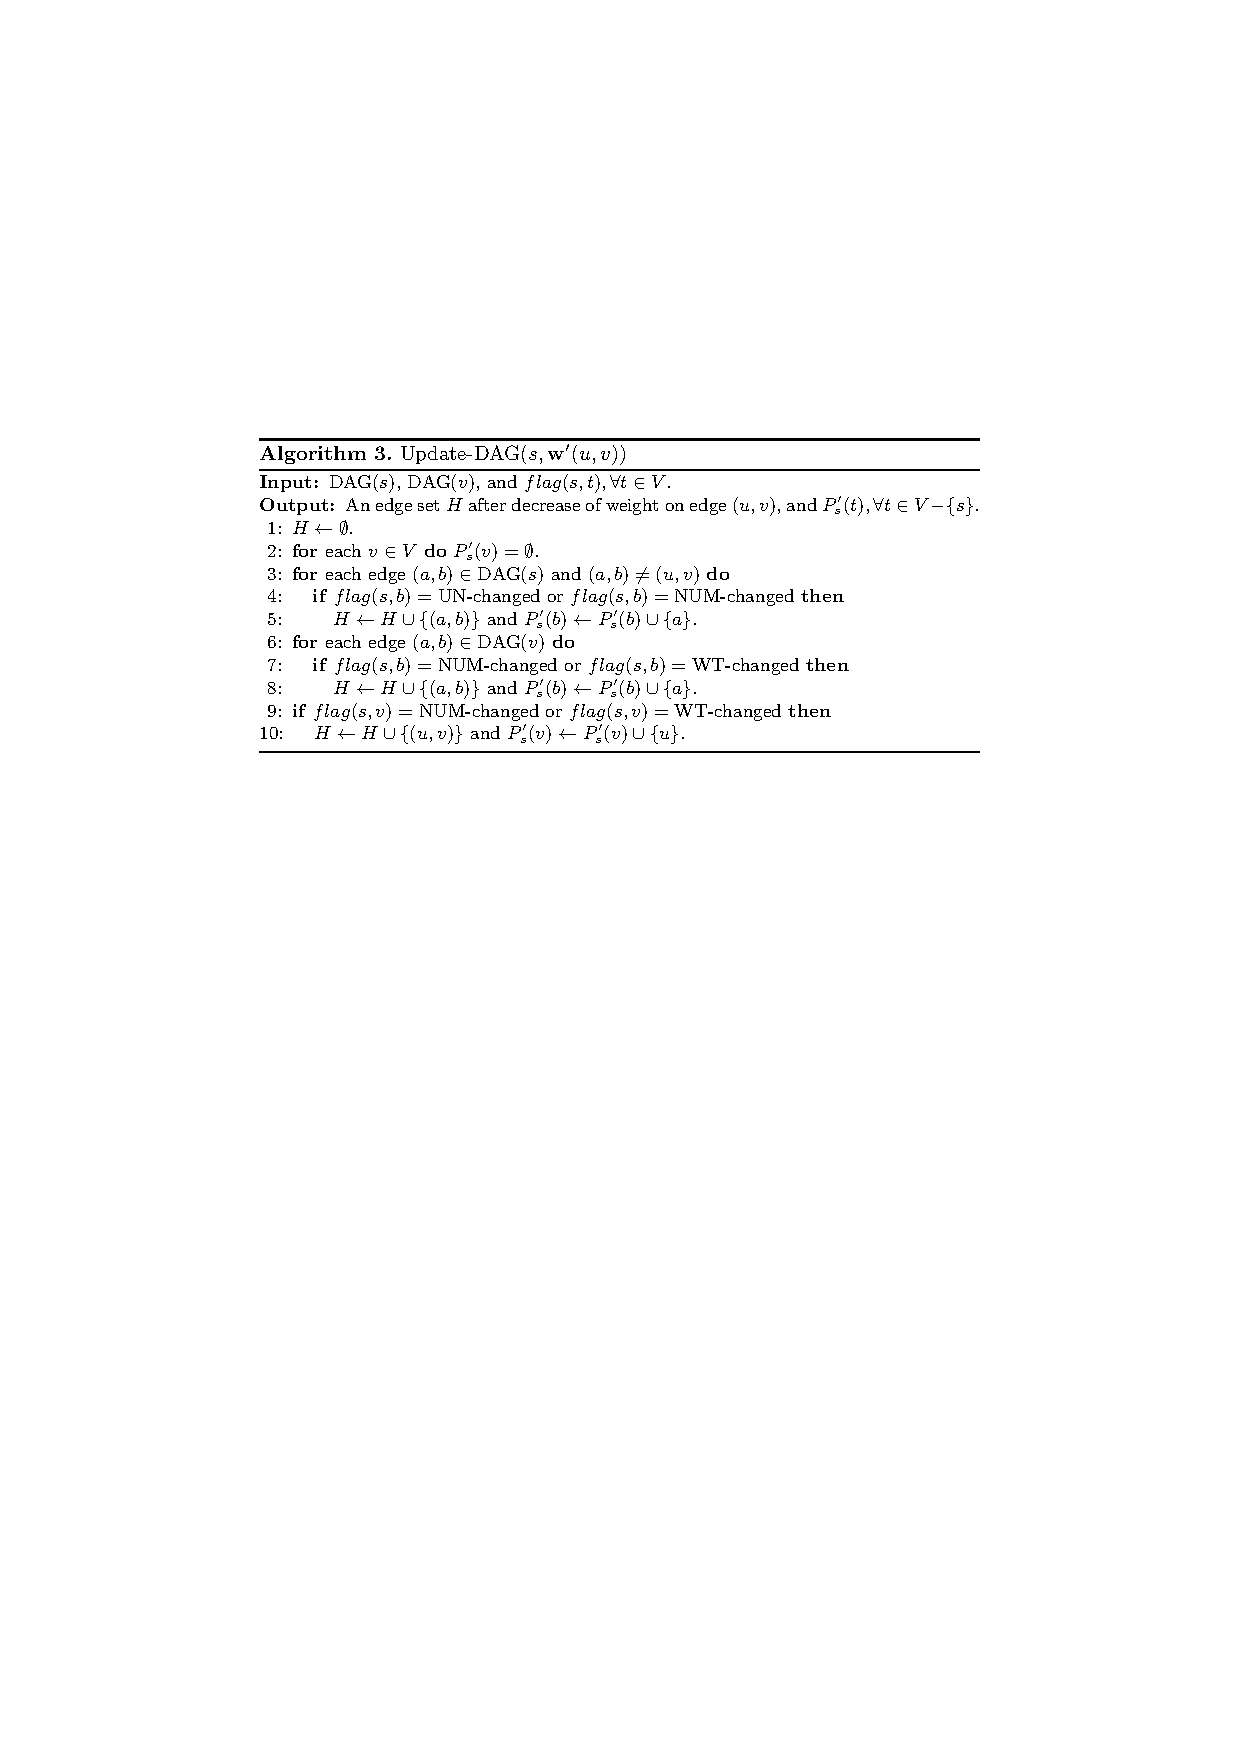
\includegraphics[width=\textwidth]{imgs/npr14-algo3}
  \end{figure}
  
\end{frame}

\begin{frame}
  \frametitle{Edge Update}

  \begin{figure}[H]
    \centering
    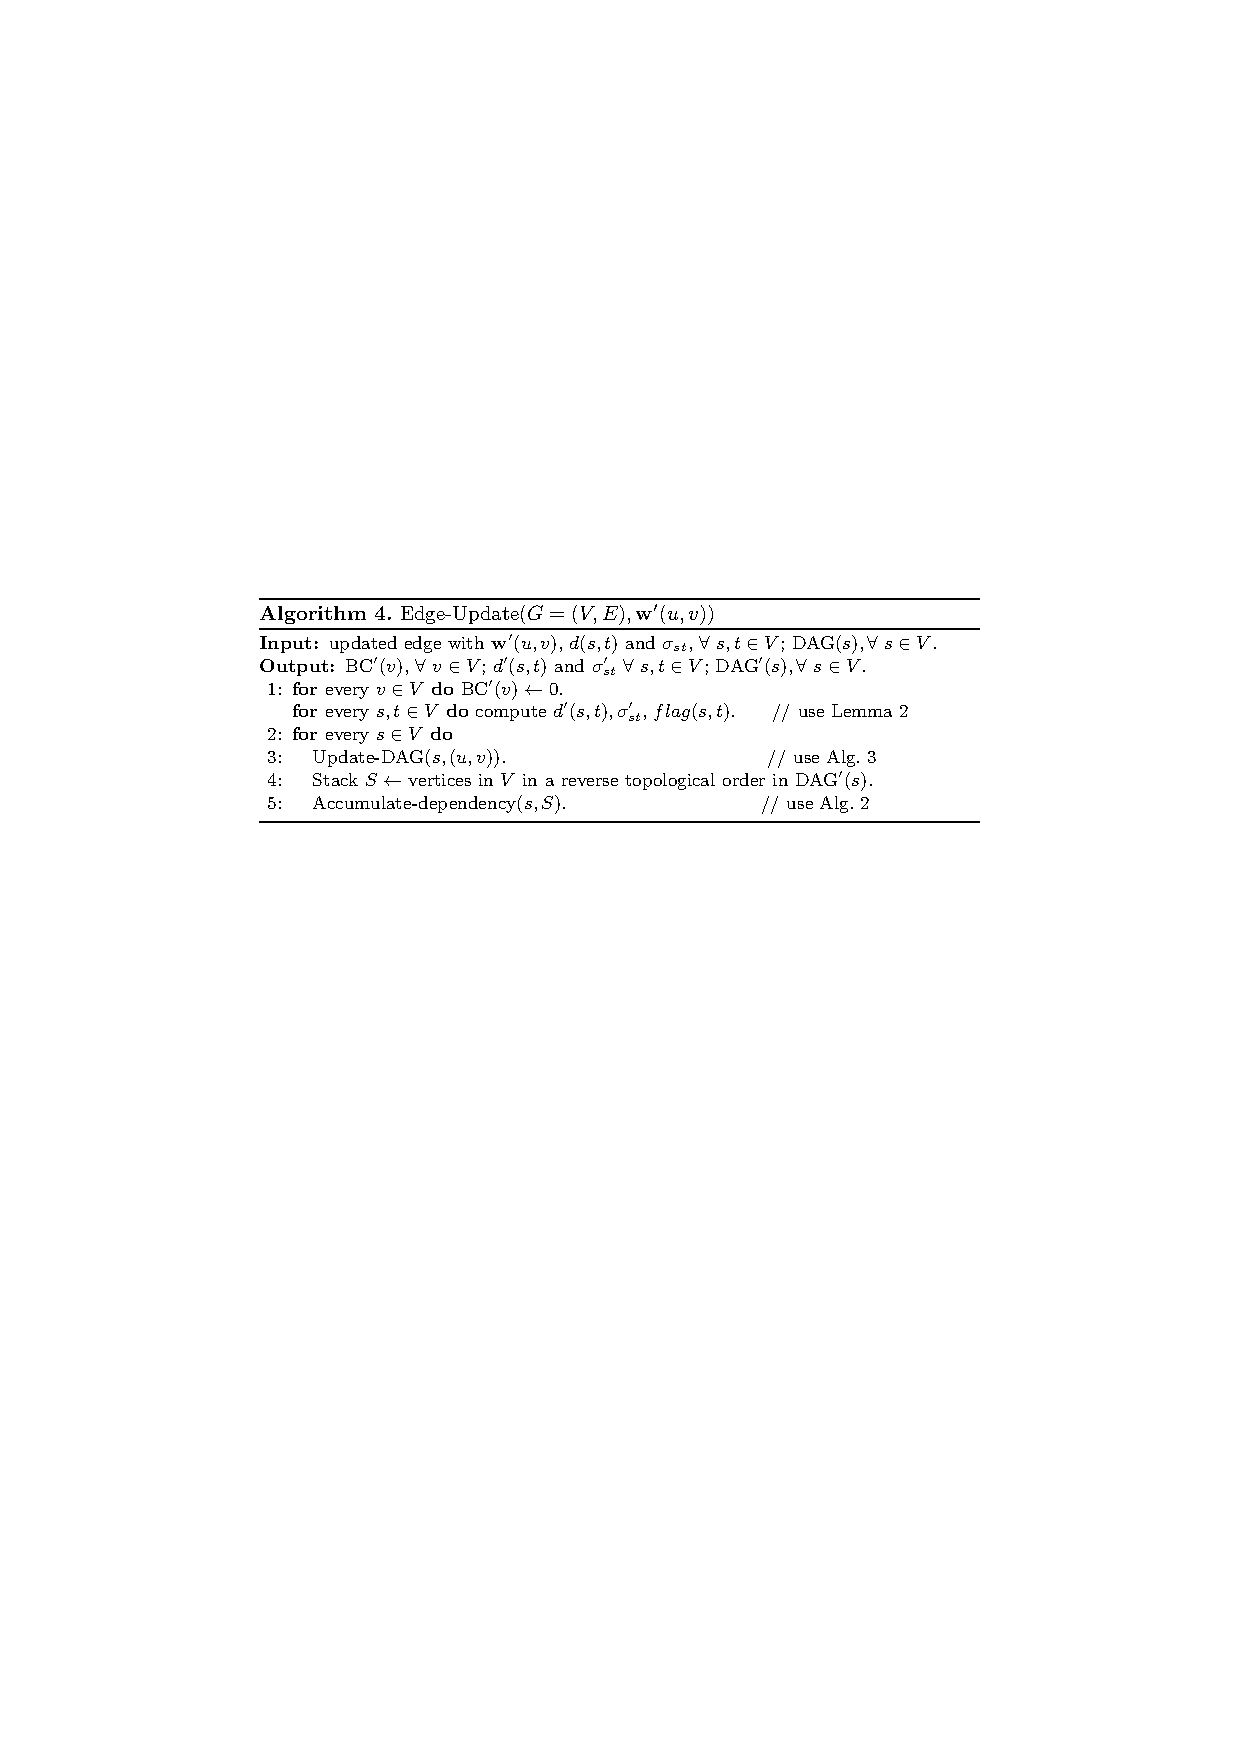
\includegraphics[width=\textwidth]{imgs/npr14-algo4}
  \end{figure}
  
\end{frame}

\begin{frame}
  \frametitle{Space-Efficient Variant $O(n^2)$}
  
  \begin{itemize}
    \item Do not store the \sssp \dag
    \item Store only $E^*$
    \item Updated \dag can be build in $O(m^*)$ time
    \begin{itemize}
      \item Time $O(m^* \times n)$
      \item Compute ${E'}^*$ from $E^*$, then $\dag'(s)$ from ${E'}^*$
    \end{itemize}
    \item Space $O(m^* + n^2)$ to store $E^*$ and $n^2$ distances $\dist(s,t)$ and shortest paths $\paths_{st}$
  \end{itemize}
  
\end{frame}

\begin{frame}
  \frametitle{Comparison}

  \begin{figure}[H]
    \centering
    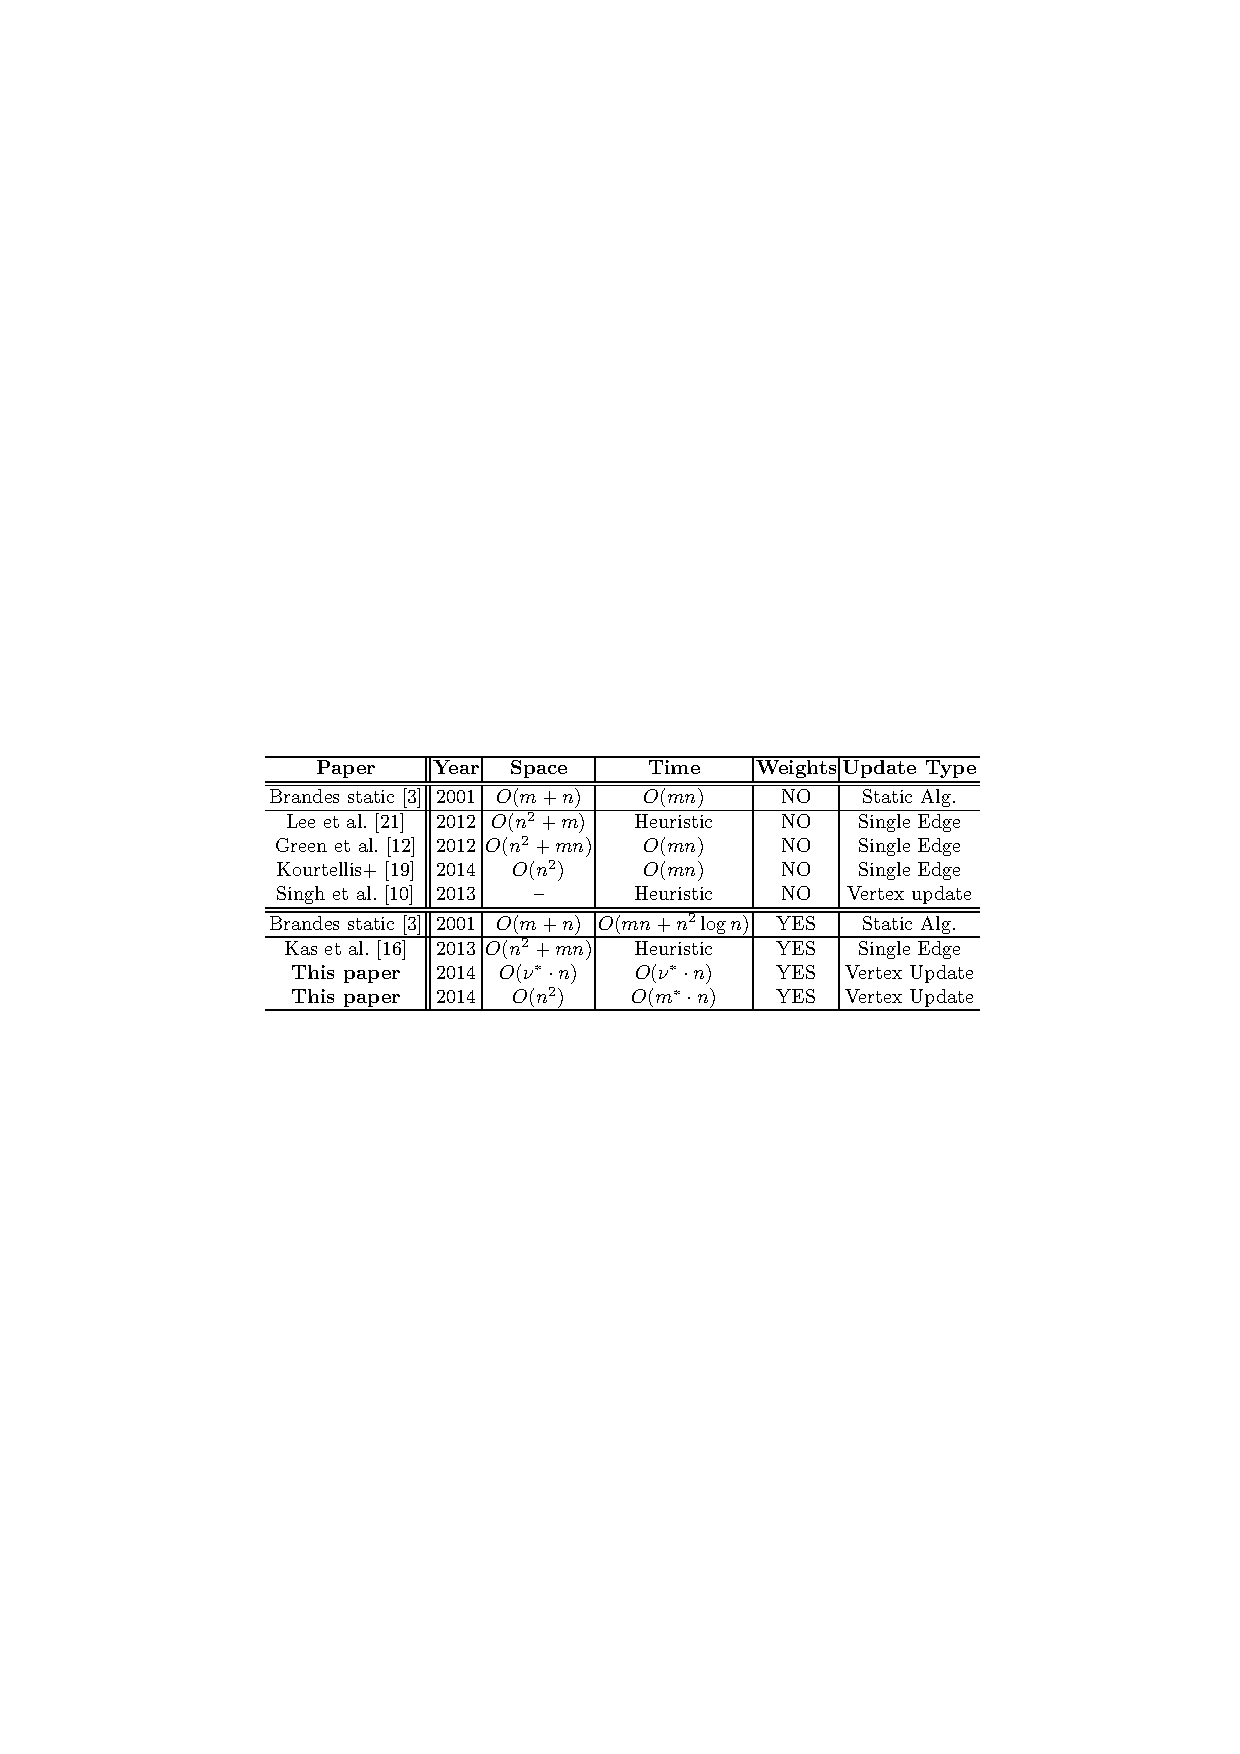
\includegraphics[width=\textwidth]{imgs/npr14-comparison}
  \end{figure}
  
\end{frame}

\begin{frame}
  \frametitle{Shortcomings}

  \begin{itemize}
    \item Not fully dynamic (no edge removal)
    \item $m^*$ can be large in practice
    \item Non-trivial to parallelize (need to access pairs of \sssp \dag at a time)
    \item Does not solve main bottleneck of most algorithms: $O(n^2)$ memory
  \end{itemize}
  
\end{frame}